\chapter{Configuration et maintenance de \ReplicaGenOne{}}\label{ch:replica-setup}

Ce chapitre concerne le combiné \ReplicaGenOne{} classique présenté à l'\autoref{fig:replica-classic}. Si votre tableau correspond à la disposition \ReplicaNextLong{}, reportez-vous au chapitre précédent.

\begin{figure}[htbp]
    \centering
    \begin{subfigure}{0.46\textwidth}
        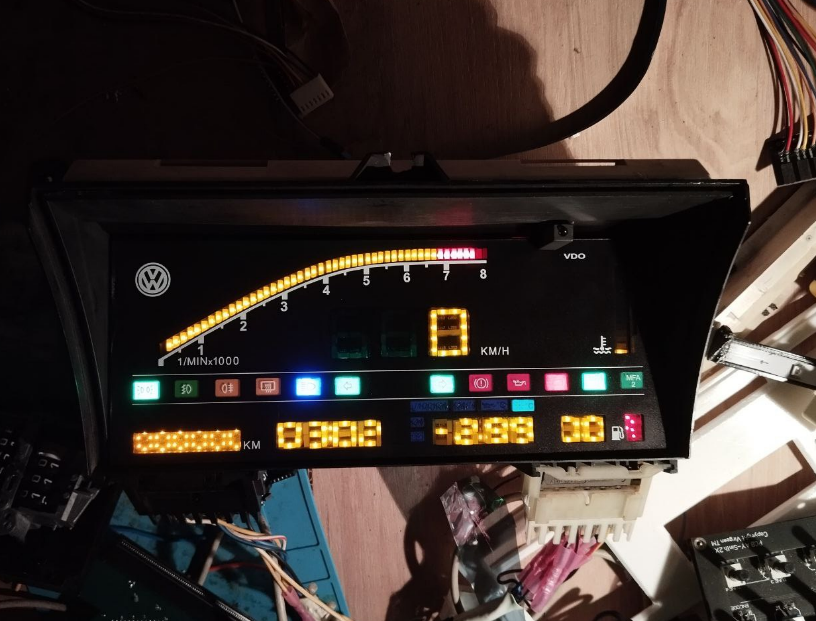
\includegraphics[width=\linewidth]{digifiz_manual/image046.png}
        \caption{\ReplicaGenOne{} classique avec encadrement carré.}
    \end{subfigure}\hfill
    \begin{subfigure}{0.46\textwidth}
        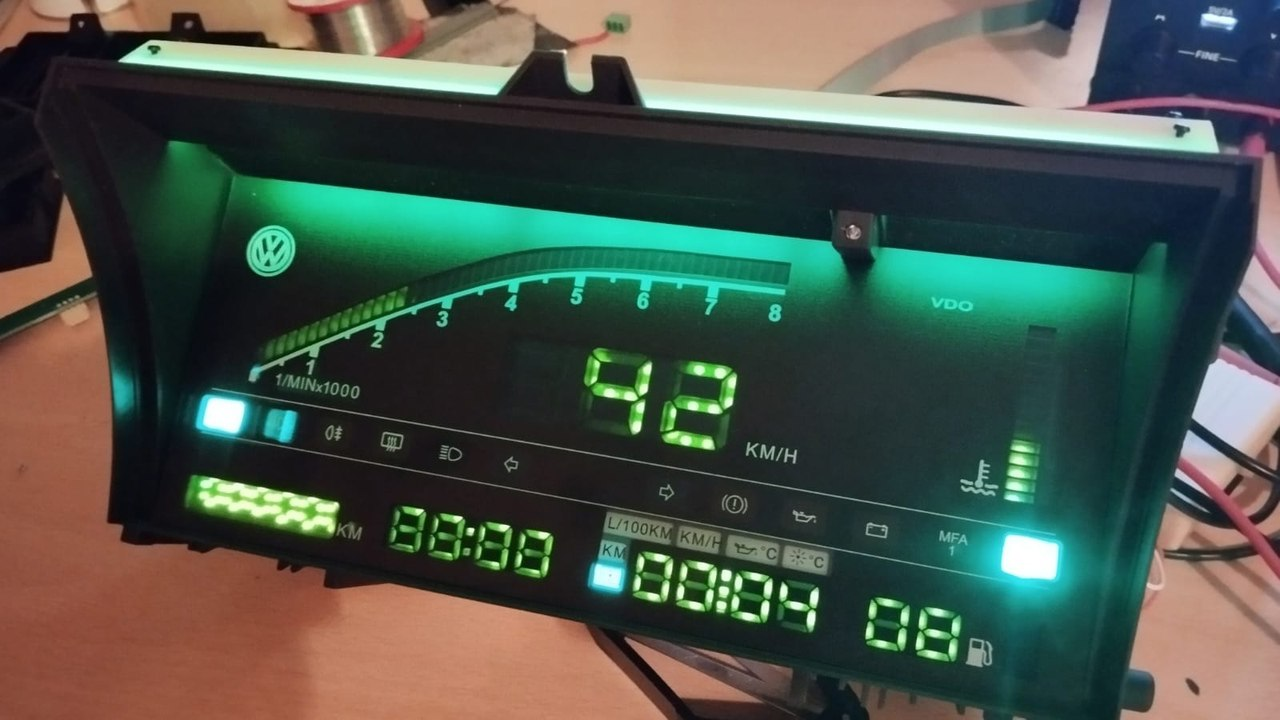
\includegraphics[width=\linewidth]{digifiz_manual/image047.png}
        \caption{Façade à angles arrondis utilisée sur les kits récents.}
    \end{subfigure}
    \caption{Aspect du tableau \ReplicaGenOne{}.}
    \label{fig:replica-classic}
\end{figure}

\section{Manipulation et entretien de l'écran}
\begin{itemize}
    \item La façade plexiglas imprimée aux UV se raye facilement. Évitez tout contact avec des objets pointus ou abrasifs.
    \item Les dommages de surface sont esthétiques et non couverts par la garantie. Demandez des pièces de rechange à PHOL-LABS Kft si le motif de l'écran est déformé.
\end{itemize}

\section{Pile de l'horloge temps réel}
Le tableau contient une horloge DS3231 alimentée par une pile CR2032 dont la durée de vie est d'environ quatre ans. Une fois déchargée, l'horloge se réinitialise à chaque mise sous tension. Retirez la façade et/ou le capot arrière, laissez les faisceaux branchés et remplacez la pile bouton. Éliminez la pile usagée conformément à la réglementation locale.

\section{Maintenance du micrologiciel avec USBasp}
Chaque kit est livré avec un cordon de programmation USBasp déjà connecté dans le boîtier (\autoref{fig:usbasp-cable}). Installez un pilote USBasp adapté avant le flashage, par exemple depuis l'adresse suivante~:
\displayurl{https://myrobot.ru/downloads/driver-usbasp-v-2.0-usb-isp-windows-7-8-10-xp.php}
Le programmateur alimente le tableau lorsqu'il est relié à un ordinateur, ce qui permet les essais sur établi.

\begin{figure}[htbp]
    \centering
    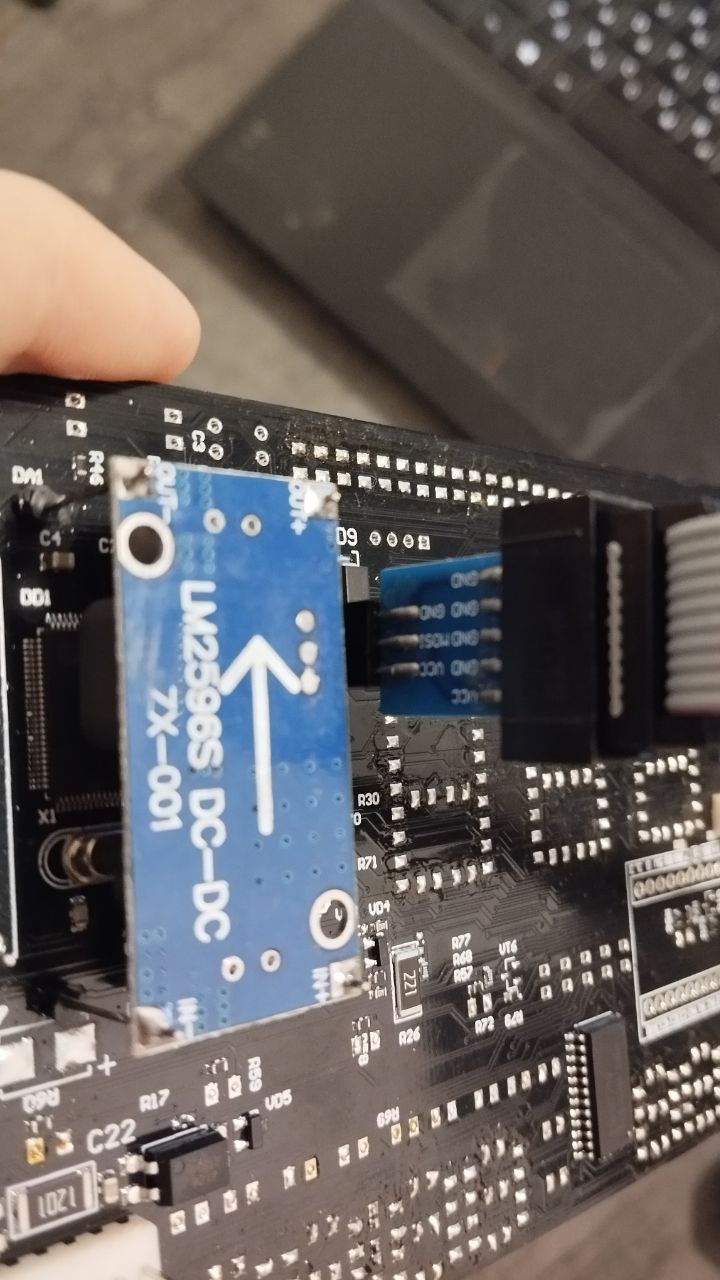
\includegraphics[width=0.32\textwidth]{digifiz_manual/image048.png}
    \caption{Orientation du faisceau USBasp dans \ReplicaGenOne{}.}
    \label{fig:usbasp-cable}
\end{figure}

Flashez le micrologiciel avec \texttt{avrdude} à l'aide de la commande ci-dessous (remplacez le nom du firmware si nécessaire)~:

\begin{verbatim}
avrdude -c usbasp -p m2560 -e \
    -U lfuse:w:0xff:m -U hfuse:w:0x99:m -U efuse:w:0xff:m \
    -U flash:w:Digifiz.ino.mega.hex
\end{verbatim}

Après un téléversement réussi, appuyez quatre à cinq fois sur le bouton tactile en façade pour initialiser les blocs mémoire. S'ils restent vides, répétez l'opération ou envoyez la commande Bluetooth \verb|252 0| pour lancer une réinitialisation usine. Des images prêtes à l'emploi sont publiées sur~:
\displayurl{https://github.com/Sgw32/DigifizReplica}

\section{Configuration Bluetooth}
La plupart des paramètres se règlent via Bluetooth depuis un téléphone Android avec l'application Serial Bluetooth Terminal. Téléchargez-la avant l'appairage~:
\displayurl{https://play.google.com/store/apps/details?id=de.kai_morich.serial_bluetooth_terminal&hl=en&gl=US}
Les appareils iOS ne peuvent pas se connecter au module Bluetooth 2.0 classique.

\begin{itemize}
    \item Associez-vous bien à l'interface Bluetooth Classic du tableau, et non à des périphériques BLE uniquement.
    \item Dans Serial Bluetooth Terminal, définissez le caractère de fin de ligne sur LF. Désactivez CR+LF avant d'envoyer des commandes.
\end{itemize}

\begin{figure}[htbp]
    \centering
    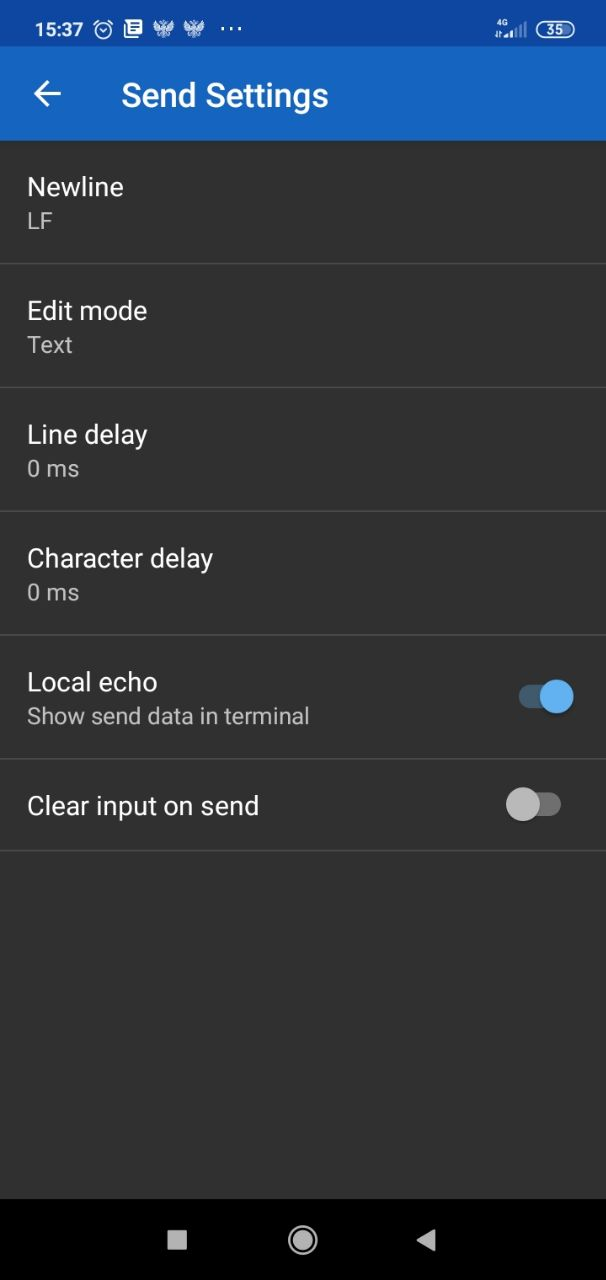
\includegraphics[width=0.32\textwidth]{digifiz_manual/image049.png}
    \caption{Configuration recommandée pour Serial Bluetooth Terminal.}
    \label{fig:sbt-settings}
\end{figure}

Saisissez les commandes sous forme de paires \verb|<nombre> <valeur>| séparées par un espace. Par exemple, pour enregistrer un odomètre de 123\,456~km, envoyez \verb|11 123456|. Ajoutez 128 au numéro d'une commande pour lire sa valeur actuelle (\verb|129 0| renvoie le coefficient de vitesse). La commande de diagnostic \verb|adc 0| affiche les lectures brutes utiles au diagnostic.

\section{Paramètres de configuration}
Les principales commandes Bluetooth figurent dans l'\autoref{tbl:replica-classic-commands}. Les paramètres par défaut des tableaux des générations~1/1.5 et~2 sont résumés à l'\autoref{tbl:replica-defaults}. N'utilisez les commandes~31--33 que sur \ReplicaNextShort{} ; elles n'ont aucun effet sur \ReplicaGenOneShort{} classique.

{\scriptsize
\begin{longtblr}[
    caption = {Commandes de configuration \ReplicaGenOne{} classique.},
    label = {tbl:replica-classic-commands},
]{
    colspec = {Q[c,0.14\linewidth] >{\ttfamily}Q[l,0.38\linewidth] Q[l]},
    rowsep = 2pt,
}
    \toprule
    \textbf{ID} & \textbf{Nom} & \textbf{Description} \\
    \midrule
    22 (ou 0) & PARAMETER\_RPMCOEFFICIENT & Facteur d'étalonnage du régime moteur. \\
    1 & PARAMETER\_SPEEDCOEFFICIENT & Facteur d'étalonnage de vitesse. \\
    2 & PARAMETER\_COOLANTTHERMISTORB & Coefficient bêta de thermistance liquide. \\
    3 & PARAMETER\_OILTHERMISTORB & Coefficient bêta de thermistance huile. \\
    4 & PARAMETER\_AIRTHERMISTORB & Coefficient bêta de thermistance ambiante. \\
    5 & PARAMETER\_TANKMINRESISTANCE & Résistance minimale de jauge (\si{\ohm}). \\
    6 & PARAMETER\_TANKMAXRESISTANCE & Résistance maximale de jauge (\si{\ohm}). \\
    7 & PARAMETER\_TAU\_COOLANT & Constante de filtrage température liquide. \\
    8 & PARAMETER\_TAU\_OIL & Constante de filtrage température huile. \\
    9 & PARAMETER\_TAU\_AIR & Constante de filtrage température ambiante. \\
    10 & PARAMETER\_TAU\_TANK & Constante de filtrage niveau carburant. \\
    11 & PARAMETER\_MILEAGE & Kilométrage total. \\
    12 & PARAMETER\_DAILY\_MILEAGE & Compteur journalier. \\
    13 & PARAMETER\_AUTO\_BRIGHTNESS & Activation du réglage automatique de luminosité. \\
    14 & PARAMETER\_BRIGHTNESS\_LEVEL & Niveau de luminosité manuel (0--15). \\
    15 & PARAMETER\_TANK\_CAPACITY & Capacité du réservoir (litres). \\
    16 & PARAMETER\_MFA\_STATE & Page MFA active. \\
    17 & PARAMETER\_BUZZER\_OFF & Désactivation du buzzer (1 coupe, 0 active). \\
    18 & PARAMETER\_MAX\_RPM & Échelle du compte-tours (8000 par défaut). \\
    19 & PARAMETER\_NORMAL\_RESISTANCE\_COOLANT & Résistance de sonde liquide à \SI{25}{\celsius}. \\
    20 & PARAMETER\_NORMAL\_RESISTANCE\_OIL & Résistance de sonde huile à \SI{25}{\celsius}. \\
    21 & PARAMETER\_NORMAL\_RESISTANCE\_AMB & Résistance de sonde ambiante à \SI{25}{\celsius}. \\
    23 & PARAMETER\_DOT\_OFF & Comportement des deux-points de l'horloge (0 clignote, 1 fixe). \\
    24 & PARAMETER\_BACKLIGHT\_ON & Allumage du rétroéclairage avec les feux de croisement. \\
    25 & PARAMETER\_M\_D\_FILTER & Constante de filtre médian (héritage). \\
    26 & PARAMETER\_COOLANT\_MAX\_R & Seuil pleine échelle de température liquide. \\
    27 & PARAMETER\_COOLANT\_MIN\_R & Seuil « 1~bar » de température liquide. \\
    31--33 & PARAMETER\_MAINCOLOR\_[RGB] & Composantes couleur interface (\ReplicaNextShort{} uniquement). \\
    37 & PARAMETER\_RPM\_FILTER & Agressivité du filtrage régime. \\
    128 & PARAMETER\_READ\_ADDITION & Addition pour lire un paramètre. \\
    255 & PARAMETER\_SET\_HOUR & Réglage des heures (24~h). \\
    254 & PARAMETER\_SET\_MINUTE & Réglage des minutes. \\
    253 & PARAMETER\_RESET\_DAILY\_MILEAGE & Remise à zéro du compteur journalier. \\
    252 & PARAMETER\_RESET\_DIGITAL & Réinitialisation usine et initialisation mémoire. \\
    \bottomrule
\end{longtblr}}

Les boutons rapides de Serial Bluetooth Terminal sont pratiques pour les actions courantes comme l'activation/désactivation de la luminosité automatique (\verb|13 0| et \verb|13 1|) ou l'écriture de valeurs de couleur. Ne dépassez \SI{60}{\percent} de luminosité que lors de tests courts afin de préserver les LED.
